% USE CASE TABLE 1: SIGN UP
 In this section there will be presented users use case tables \ldots
\begin{table}[H]
    \centering
    \begin{tabular}[c]{|l|p{0.75\textwidth}|}
        \hline % ---------------------------------------------------------------------
    	\textsc{id}                 &   1\\
    	\hline % ---------------------------------------------------------------------
    	\textsc{Name}               &   Sign up User with email\\
    	\hline % ---------------------------------------------------------------------
    	\textsc{Actors}             &   User\\
    	\hline % ---------------------------------------------------------------------
    	\textsc{Entry conditions}   &   User has opened the Web page OR User has downloaded and opened the application on his smartphone\\
    	\hline % ---------------------------------------------------------------------
    	\textsc{Input}   &   Email to use for the registration\\
    	\hline % ---------------------------------------------------------------------
    	\textsc{Event flow}         &   \footnotesize
            	                        \begin{itemize}
                                    	    \item The system displays the “Sign in” page
                                            \item User clicks on “Sign up”
                                            \item The system displays two fields: email and password
                                            \item User inserts the data and accepts the “Terms of services”
                                            \item User clicks on the “Confirm” button
                                            \item The system displays the acceptance of the registration and invites User to go to his inbox in order to confirm the registration
                                            \item User opens his inbox, checks the email and clicks on the confirmation link

                                        \end{itemize}\\
        \hline % ---------------------------------------------------------------------
        \textsc{Exit conditions}    &  User registration has been successful: user data are stored in the system’s database. User can now login with his credentials\\
    	\hline % ---------------------------------------------------------------------
    	\textsc{Output}             &  \begin{itemize}
    	    \item User’s email is stored in the system’s database
            \item User receives the confirmation email

    	\end{itemize}\\
    	\hline % ---------------------------------------------------------------------
    	\textsc{Exceptions}         &  \begin{itemize}
    	    \item User inserts an email which is already stored in the database. So, after User clicks on “Confirm”, the system displays an error page which tells that User is already registered to the service and invites him to login with that email
            \item User inserts an invalid email. So, after User clicks on “Confirm”, the system displays the same sign up page with an error message, which suggests User to check the inserted email or to change it

    	\end{itemize}\\
    	\hline % ---------------------------------------------------------------------
        
    \end{tabular}
    \caption{\label{tab:responsible_area_insertion}User caption \textnumero 1}
\end{table}

\begin{figure}[H]
    \centering
    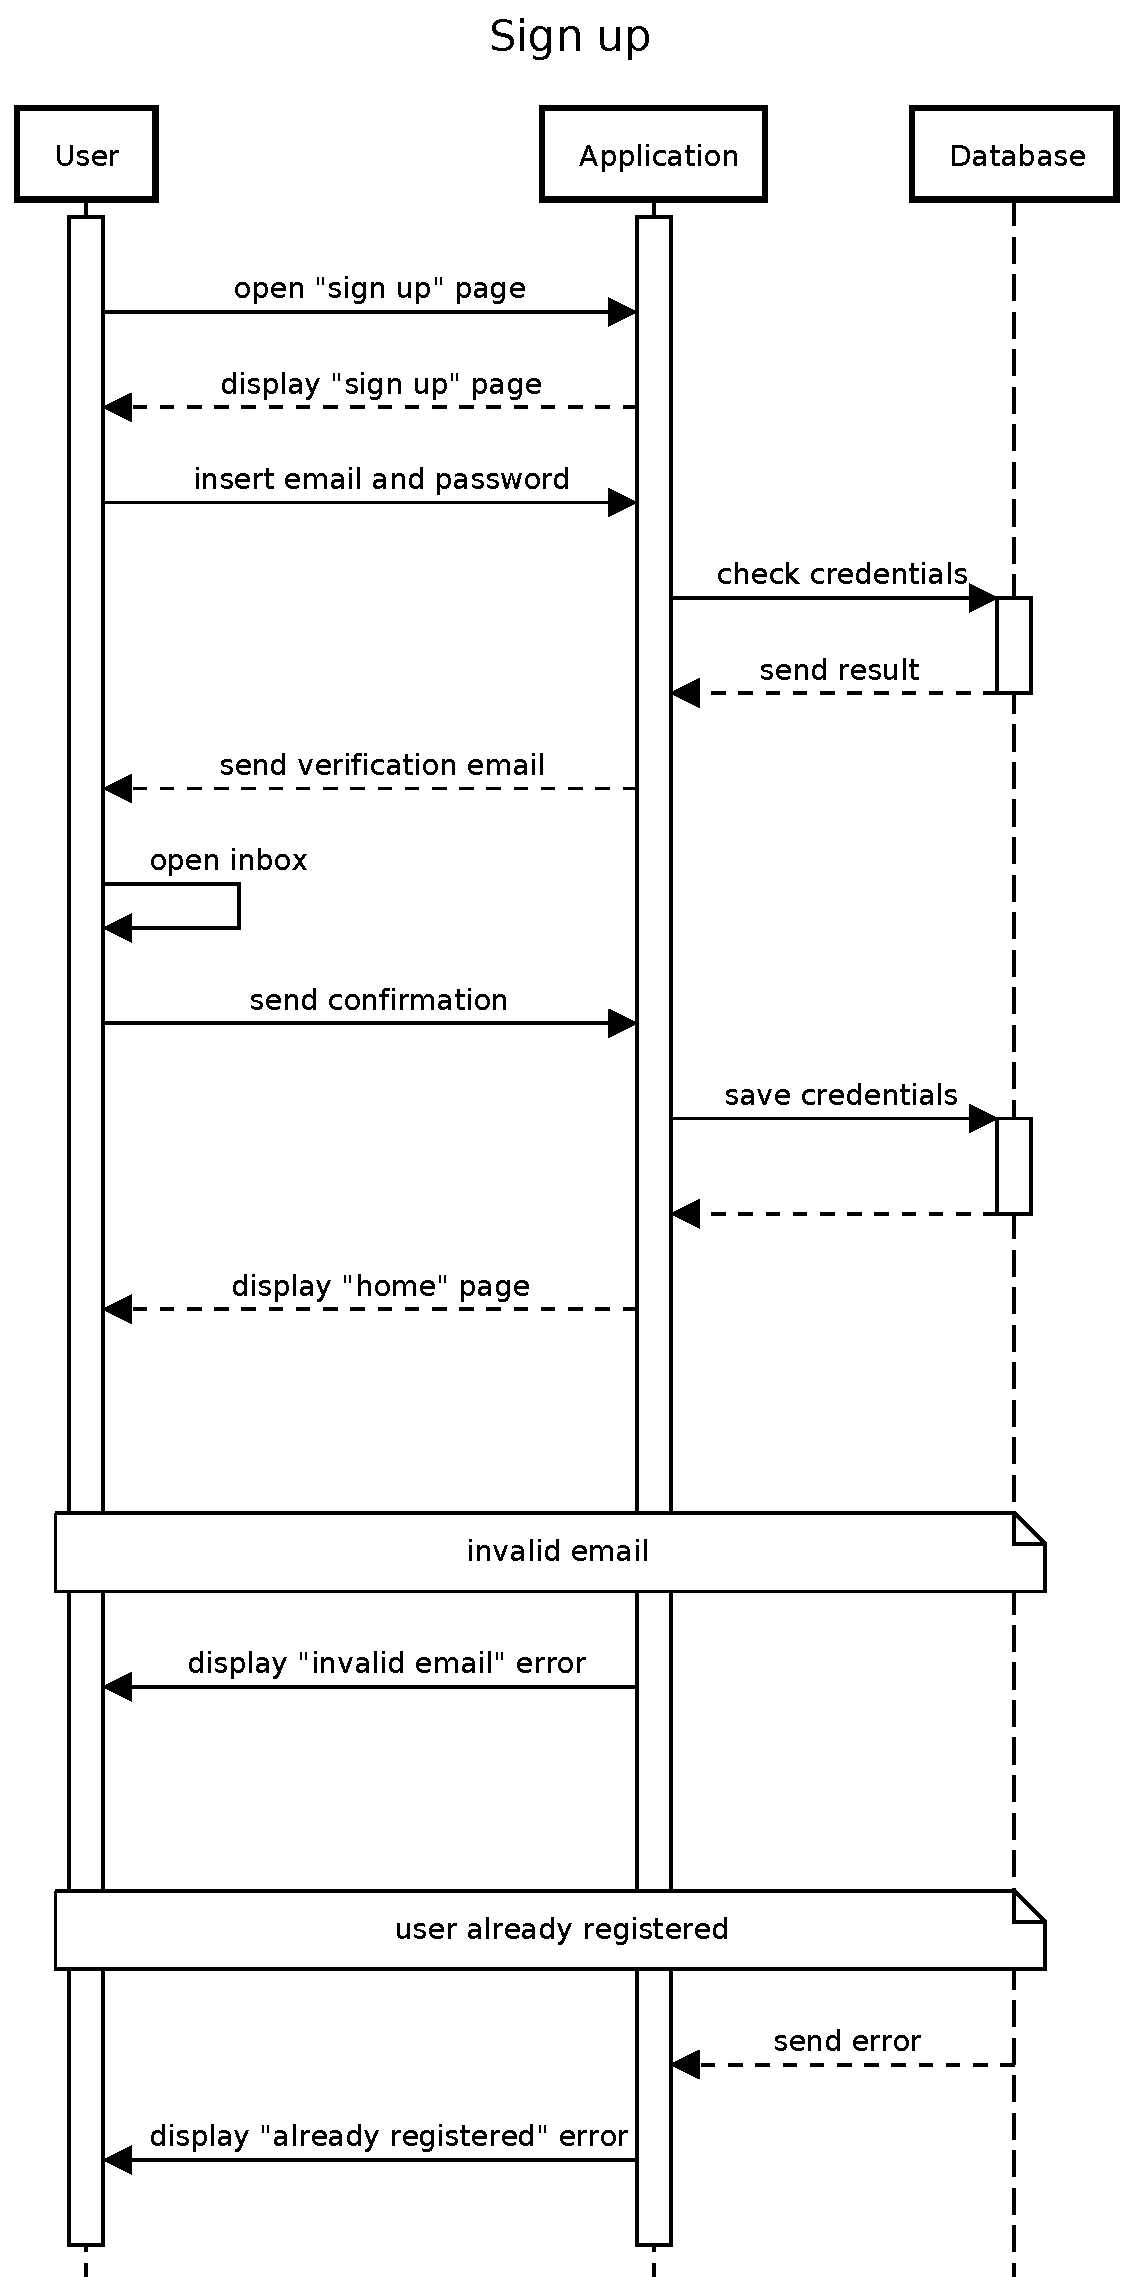
\includegraphics[scale=0.5]{Images/Sequence diagrams/User - sign up.pdf}
    \caption{Caption}
    \label{fig:my_label}
\end{figure}

\begin{table}[H]
    \centering
    \begin{tabular}[c]{|l|p{0.75\textwidth}|}
        \hline % ---------------------------------------------------------------------
    	\textsc{id}                 &   2\\
    	\hline % ---------------------------------------------------------------------
    	\textsc{Name}               &   Login User\\
    	\hline % ---------------------------------------------------------------------
    	\textsc{Actors}             &   User\\
    	\hline % ---------------------------------------------------------------------
    	\textsc{Entry conditions}   &   User has opened the Web page OR User has downloaded and opened the application on his smartphone\\
    	\hline % ---------------------------------------------------------------------
    	\textsc{Input}   &   User’s valid email and password\\
    	\hline % ---------------------------------------------------------------------
    	\textsc{Event flow}         &   \footnotesize
            	                        \begin{itemize}
                                    	    \item The system displays the “Login” page
                                            \item User inserts his credentials (email, password) and clicks the “Login” button
                                            \item The system checks the correctness of the inserted credentials
                                            \item The system displays the home page


                                        \end{itemize}\\
        \hline % ---------------------------------------------------------------------
        \textsc{Exit conditions}    &  User is logged in\\
    	\hline % ---------------------------------------------------------------------
    	\textsc{Output}             &  \begin{itemize}
    	    \item User inserts a wrong combination of email and password. The system displays the same page with an error message.

    	\end{itemize}\\
    	\hline % ---------------------------------------------------------------------
    	\textsc{Exceptions}         &  \begin{itemize}
    	    \item User inserts an email which is already stored in the database. So, after User clicks on “Confirm”, the system displays an error page which tells that User is already registered to the service and invites him to login with that email
            \item User inserts an invalid email. So, after User clicks on “Confirm”, the system displays the same sign up page with an error message, which suggests User to check the inserted email or to change it

    	\end{itemize}\\
    	\hline % ---------------------------------------------------------------------
        
    \end{tabular}
    \caption{\label{tab:responsible_area_insertion}User caption \textnumero 2}
\end{table}

\begin{figure}[H]
    \centering
    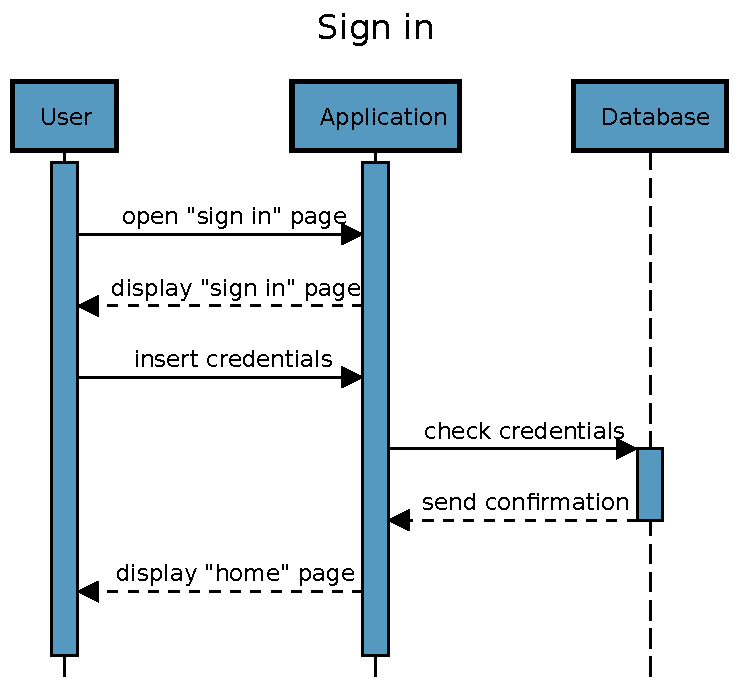
\includegraphics[scale=0.5]{Images/Sequence diagrams/User - sign in.pdf}
    \caption{Caption}
    \label{fig:my_label}
\end{figure}
